\documentclass{beamer} % imports amsmath symbols

\usepackage{mathleague}

\newcommand{\contestproblemset}{12128}
\newcommand{\roundname}{Sprint}
\newcommand{\problemnumber}{29}

\begin{document}

\begin{frame} % Title Page
  \titlepage
\end{frame}

%\begin{frame} % Page 2
%  \frametitle{Table of Contents}
%  \tableofcontents[hideallsubsections]
%\end{frame}

\section{Problem}

\subsection*{Identify the objective.}
%\stepcounter{subsection}

\begin{frame}
  \frametitle{}
  In $\triangle XYZ$, side $XY$ has length $4$ and side $YZ$ has length $3$. Point $W$ lies on side $XZ$ such that the length of segment $YW$ is $2$, and the length of segment $XW$ is twice the length of segment $WZ$. What is the square of the length of side $XZ$?
  \begin{center}
    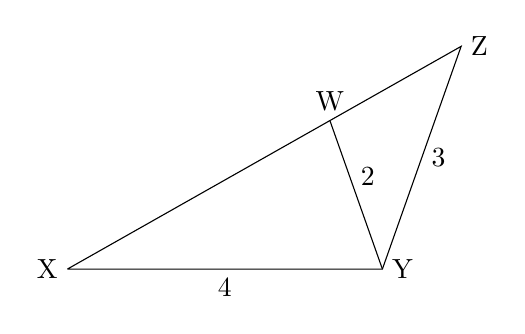
\begin{tikzpicture}[scale=1.0]
        \draw (0,0) -- (4,0) node [right] {Y} node [midway,below] {4} -- (5,2.82842712) node [right] {Z} node [midway,right] {3} -- (0,0) node [left] {X};
        \draw (4,0) -- (3.33333333,1.88561808) node [above] {W} node [midway, above] {\;\;\;2};
    \end{tikzpicture}
  \end{center}
\end{frame}

\section{Solution}

\subsection*{Compute $XZ^2$.}

\begin{comment}
\begin{frame}
  \begin{center}
    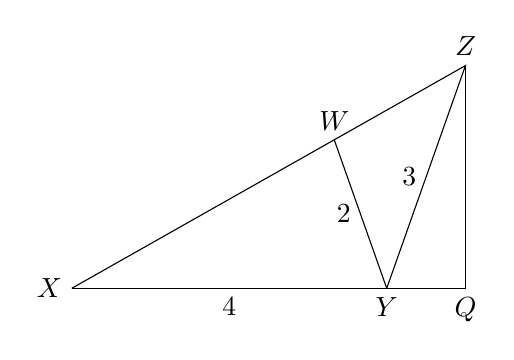
\begin{tikzpicture}[scale=1]
      \draw (0,0) -- (4,0) node [midway,below] {$4$};
      \draw (4,0) -- (5,2.82842712) node [midway,left] {$3$} -- (0,0);
      \draw (4,0) -- (3.33333333,1.88561808) node [midway, left] {$2$};
      \draw (3.33333333,1.88561808) node [above] {$W$};
      \draw (0,0) node [left] {$X$};
      \draw (4,0) node [below] {$Y$};
      \draw (5,2.82842712) node [above] {$Z$};
      \draw (5,0) node [below] {$Q$};

      \draw (4,0)--(5,0)--(5,2.82842712);
      \draw (5,2.82842712)--(5,0);
      \coordinate (Z) at (5,2.82842712);
      \coordinate (Q) at (5,0);
      \coordinate (Y) at (4,0);
      \tkzMarkRightAngle(Z,Q,Y)
    \end{tikzpicture}
  \end{center}
\end{frame}

\begin{frame}
  \begin{center}
    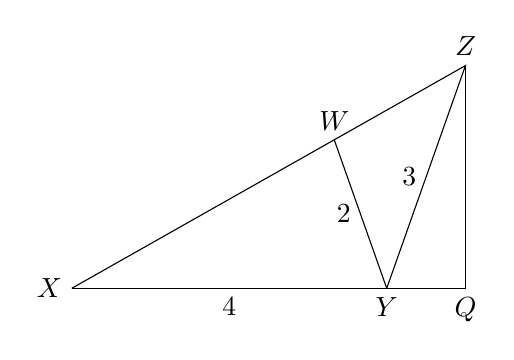
\begin{tikzpicture}[scale=1]
      \draw (0,0) -- (4,0) node [midway,below] {$4$};
      \draw (4,0) -- (5,2.82842712) node [midway,left] {$3$} -- (0,0);
      \draw (4,0) -- (3.33333333,1.88561808) node [midway, left] {$2$};
      \draw (3.33333333,1.88561808) node [above] {$W$};
      \draw (0,0) node [left] {$X$};
      \draw (4,0) node [below] {$Y$};
      \draw (5,2.82842712) node [above] {$Z$};
      \draw (5,0) node [below] {$Q$};

      \draw (4,0)--(5,0)--(5,2.82842712);
      \draw (5,2.82842712)--(5,0);
      \coordinate (Z) at (5,2.82842712);
      \coordinate (Q) at (5,0);
      \coordinate (Y) at (4,0);
      \tkzMarkRightAngle(Z,Q,Y)
    \end{tikzpicture}
  \end{center}
  Idea: $XZ^2=XQ^2+QZ^2$ by Pythagorean theorem
\end{frame}

\begin{frame}
  \begin{center}
    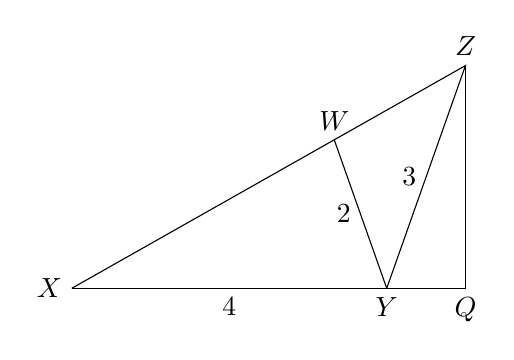
\begin{tikzpicture}[scale=1]
      \draw (0,0) -- (4,0) node [midway,below] {$4$};
      \draw (4,0) -- (5,2.82842712) node [midway,left] {$3$} -- (0,0);
      \draw (4,0) -- (3.33333333,1.88561808) node [midway, left] {$2$};
      \draw (3.33333333,1.88561808) node [above] {$W$};
      \draw (0,0) node [left] {$X$};
      \draw (4,0) node [below] {$Y$};
      \draw (5,2.82842712) node [above] {$Z$};
      \draw (5,0) node [below] {$Q$};

      \draw (4,0)--(5,0)--(5,2.82842712);
      \draw (5,2.82842712)--(5,0);
      \coordinate (Z) at (5,2.82842712);
      \coordinate (Q) at (5,0);
      \coordinate (Y) at (4,0);
      \tkzMarkRightAngle(Z,Q,Y)
    \end{tikzpicture}
  \end{center}
  Idea: $XZ^2=XQ^2+(YZ^2-YQ^2)$ by Pythagorean theorem
\end{frame}

\begin{frame}
  \begin{center}
    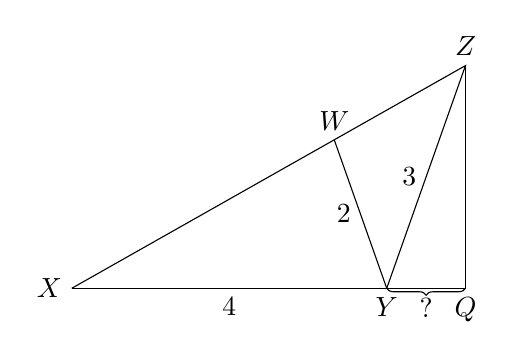
\begin{tikzpicture}[scale=1]
      \draw (0,0) -- (4,0) node [midway,below] {$4$};
      \draw (4,0) -- (5,2.82842712) node [midway,left] {$3$} -- (0,0);
      \draw (4,0) -- (3.33333333,1.88561808) node [midway, left] {$2$};
      \draw (3.33333333,1.88561808) node [above] {$W$};
      \draw (0,0) node [left] {$X$};
      \draw (4,0) node [below] {$Y$};
      \draw (5,2.82842712) node [above] {$Z$};
      \draw (5,0) node [below] {$Q$};

      \draw (4,0)--(5,0)--(5,2.82842712);
      \draw (5,2.82842712)--(5,0);
      \coordinate (Z) at (5,2.82842712);
      \coordinate (Q) at (5,0);
      \coordinate (Y) at (4,0);
      \tkzMarkRightAngle(Z,Q,Y)

      \draw [decoration={brace,mirror,raise=0cm},decorate
      ] (4,0) -- (5,0) node [midway,below=0.0cm] {$?$};
    \end{tikzpicture}
  \end{center}
  Idea: $XZ^2=XQ^2+(YZ^2-YQ^2)$ by Pythagorean theorem
\end{frame}
\end{comment}

\begin{frame}
  \begin{center}
    \begin{tikzpicture}[scale=1]
      \draw (0,0) -- (4,0) node [midway,below] {$4$};
      \draw (4,0) -- (5,2.82842712) node [midway,left] {$3$} -- (0,0);
      \draw (4,0) -- (3.33333333,1.88561808) node [midway, left] {$2$};
      \draw (3.33333333,1.88561808) node [above] {$W$};
      \draw (0,0) node [left] {$X$};
      \draw (4,0) node [below] {$Y$};
      \draw (5,2.82842712) node [above] {$Z$};
    \end{tikzpicture}
  \end{center}
\end{frame}

\begin{frame}
  \begin{center}
    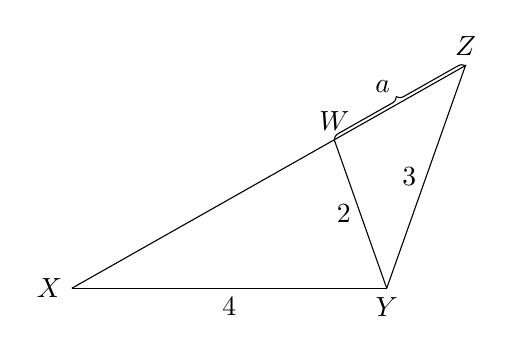
\begin{tikzpicture}[scale=1]
      \draw (0,0) -- (4,0) node [midway,below] {$4$};
      \draw (4,0) -- (5,2.82842712) node [midway,left] {$3$} -- (0,0);
      \draw (4,0) -- (3.33333333,1.88561808) node [midway, left] {$2$};
      \draw (3.33333333,1.88561808) node [above] {$W$};
      \draw (0,0) node [left] {$X$};
      \draw (4,0) node [below] {$Y$};
      \draw (5,2.82842712) node [above] {$Z$};
      \draw [decoration={brace,raise=0.0cm},decorate] (3.33333333,1.88561808)--(5,2.82842712) node [midway,above left] {$a$};
    \end{tikzpicture}
  \end{center}
\end{frame}

\begin{frame}
  \begin{center}
    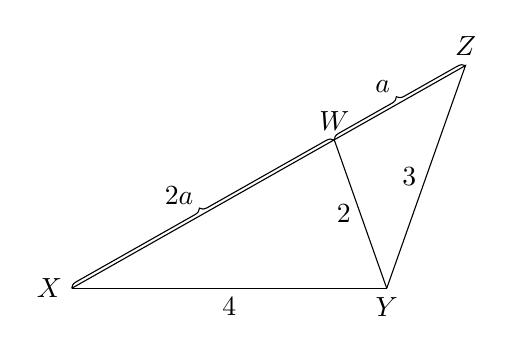
\begin{tikzpicture}[scale=1]
      \draw (0,0) -- (4,0) node [midway,below] {$4$};
      \draw (4,0) -- (5,2.82842712) node [midway,left] {$3$} -- (0,0);
      \draw (4,0) -- (3.33333333,1.88561808) node [midway, left] {$2$};
      \draw (3.33333333,1.88561808) node [above] {$W$};
      \draw (0,0) node [left] {$X$};
      \draw (4,0) node [below] {$Y$};
      \draw (5,2.82842712) node [above] {$Z$};
      \draw [decoration={brace,raise=0.0cm},decorate] (3.33333333,1.88561808)--(5,2.82842712) node [midway,above left] {$a$};
      \draw [decoration={brace,raise=0.0cm},decorate] (0,0)--(3.33333333,1.88561808) node [midway,above left] {$2a$};
    \end{tikzpicture}
  \end{center}
\end{frame}

\begin{frame}
  \begin{center}
    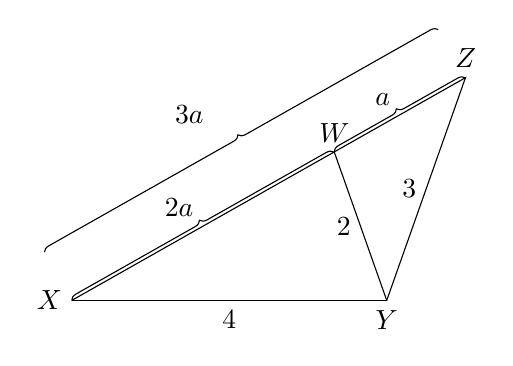
\begin{tikzpicture}[scale=1]
      \draw (0,0) -- (4,0) node [midway,below] {$4$};
      \draw (4,0) -- (5,2.82842712) node [midway,left] {$3$} -- (0,0);
      \draw (4,0) -- (3.33333333,1.88561808) node [midway, left] {$2$};
      \draw (3.33333333,1.88561808) node [above] {$W$};
      \draw (0,0) node [left] {$X$};
      \draw (4,0) node [below] {$Y$};
      \draw (5,2.82842712) node [above] {$Z$};
      \draw [decoration={brace,raise=0.0cm},decorate] (3.33333333,1.88561808)--(5,2.82842712) node [midway,above left] {$a$};
      \draw [decoration={brace,raise=0.0cm},decorate] (0,0)--(3.33333333,1.88561808) node [midway,above left] {$2a$};
      \draw [decoration={brace,raise=20pt},decorate] (0,0)--(5,2.82842712) node [midway,above left=20pt] {$3a$};
    \end{tikzpicture}
  \end{center}
\end{frame}

\begin{frame}
  \begin{center}
    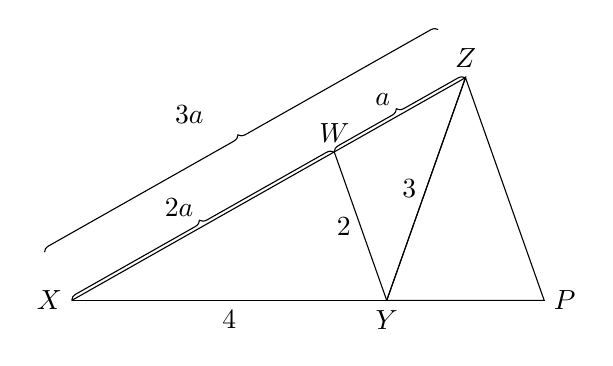
\begin{tikzpicture}[scale=1]
      \draw (0,0) -- (4,0) node [midway,below] {$4$};
      \draw (4,0) -- (5,2.82842712) node [midway,left] {$3$} -- (0,0);
      \draw (4,0) -- (3.33333333,1.88561808) node [midway, left] {$2$};
      \draw (3.33333333,1.88561808) node [above] {$W$};
      \draw (0,0) node [left] {$X$};
      \draw (4,0) node [below] {$Y$};
      \draw (5,2.82842712) node [above] {$Z$};
      \draw [decoration={brace,raise=0.0cm},decorate] (3.33333333,1.88561808)--(5,2.82842712) node [midway,above left] {$a$};
      \draw [decoration={brace,raise=0.0cm},decorate] (0,0)--(3.33333333,1.88561808) node [midway,above left] {$2a$};
      \draw [decoration={brace,raise=20pt},decorate] (0,0)--(5,2.82842712) node [midway,above left=20pt] {$3a$};

      \draw (6,0) node [right] {$P$};
      \draw (4,0)--(6,0)--(5,2.82842712)--cycle;
    \end{tikzpicture}
  \end{center}
\end{frame}

\begin{frame}
  \begin{center}
    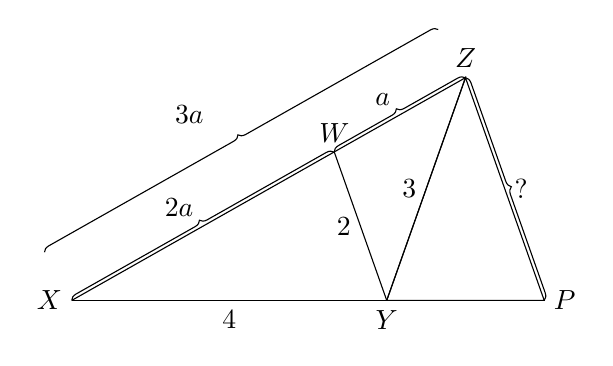
\begin{tikzpicture}[scale=1]
      \draw (0,0) -- (4,0) node [midway,below] {$4$};
      \draw (4,0) -- (5,2.82842712) node [midway,left] {$3$} -- (0,0);
      \draw (4,0) -- (3.33333333,1.88561808) node [midway, left] {$2$};
      \draw (3.33333333,1.88561808) node [above] {$W$};
      \draw (0,0) node [left] {$X$};
      \draw (4,0) node [below] {$Y$};
      \draw (5,2.82842712) node [above] {$Z$};
      \draw [decoration={brace,raise=0.0cm},decorate] (3.33333333,1.88561808)--(5,2.82842712) node [midway,above left] {$a$};
      \draw [decoration={brace,raise=0.0cm},decorate] (0,0)--(3.33333333,1.88561808) node [midway,above left] {$2a$};
      \draw [decoration={brace,raise=20pt},decorate] (0,0)--(5,2.82842712) node [midway,above left=20pt] {$3a$};

      \draw (6,0) node [right] {$P$};
      \draw (4,0)--(6,0)--(5,2.82842712)--cycle;
      \draw [decoration={brace,raise=0.0cm},decorate] (5,2.82842712)--(6,0) node [midway,right] {$?$};
    \end{tikzpicture}
  \end{center}
\end{frame}

\begin{frame}
  \begin{center}
    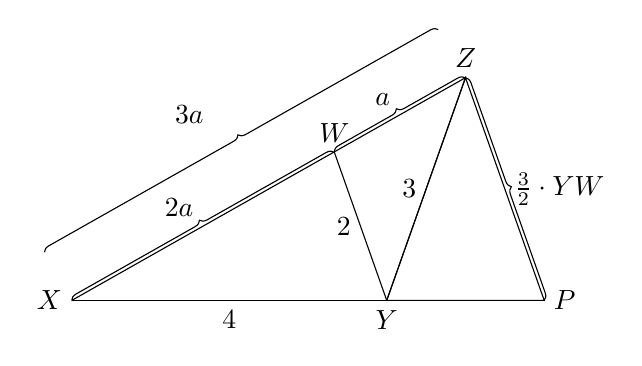
\begin{tikzpicture}[scale=1]
      \draw (0,0) -- (4,0) node [midway,below] {$4$};
      \draw (4,0) -- (5,2.82842712) node [midway,left] {$3$} -- (0,0);
      \draw (4,0) -- (3.33333333,1.88561808) node [midway, left] {$2$};
      \draw (3.33333333,1.88561808) node [above] {$W$};
      \draw (0,0) node [left] {$X$};
      \draw (4,0) node [below] {$Y$};
      \draw (5,2.82842712) node [above] {$Z$};
      \draw [decoration={brace,raise=0.0cm},decorate] (3.33333333,1.88561808)--(5,2.82842712) node [midway,above left] {$a$};
      \draw [decoration={brace,raise=0.0cm},decorate] (0,0)--(3.33333333,1.88561808) node [midway,above left] {$2a$};
      \draw [decoration={brace,raise=20pt},decorate] (0,0)--(5,2.82842712) node [midway,above left=20pt] {$3a$};

      \draw (6,0) node [right] {$P$};
      \draw (4,0)--(6,0)--(5,2.82842712)--cycle;
      \draw [decoration={brace,raise=0.0cm},decorate] (5,2.82842712)--(6,0) node [midway,right] {$\frac{3}{2}\cdot YW$};
    \end{tikzpicture}
  \end{center}
\end{frame}

\begin{frame}
  \begin{center}
    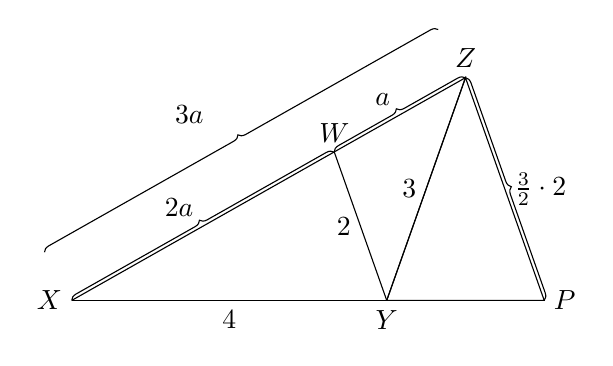
\begin{tikzpicture}[scale=1]
      \draw (0,0) -- (4,0) node [midway,below] {$4$};
      \draw (4,0) -- (5,2.82842712) node [midway,left] {$3$} -- (0,0);
      \draw (4,0) -- (3.33333333,1.88561808) node [midway, left] {$2$};
      \draw (3.33333333,1.88561808) node [above] {$W$};
      \draw (0,0) node [left] {$X$};
      \draw (4,0) node [below] {$Y$};
      \draw (5,2.82842712) node [above] {$Z$};
      \draw [decoration={brace,raise=0.0cm},decorate] (3.33333333,1.88561808)--(5,2.82842712) node [midway,above left] {$a$};
      \draw [decoration={brace,raise=0.0cm},decorate] (0,0)--(3.33333333,1.88561808) node [midway,above left] {$2a$};
      \draw [decoration={brace,raise=20pt},decorate] (0,0)--(5,2.82842712) node [midway,above left=20pt] {$3a$};

      \draw (6,0) node [right] {$P$};
      \draw (4,0)--(6,0)--(5,2.82842712)--cycle;
      \draw [decoration={brace,raise=0.0cm},decorate] (5,2.82842712)--(6,0) node [midway,right] {$\frac{3}{2}\cdot 2$};
    \end{tikzpicture}
  \end{center}
\end{frame}

\begin{frame}
  \begin{center}
    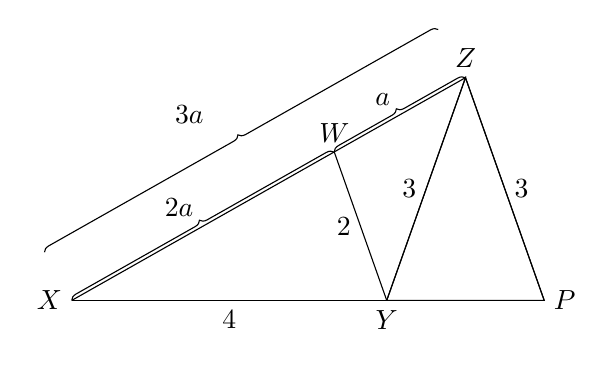
\begin{tikzpicture}[scale=1]
      \draw (0,0) -- (4,0) node [midway,below] {$4$};
      \draw (4,0) -- (5,2.82842712) node [midway,left] {$3$} -- (0,0);
      \draw (4,0) -- (3.33333333,1.88561808) node [midway, left] {$2$};
      \draw (3.33333333,1.88561808) node [above] {$W$};
      \draw (0,0) node [left] {$X$};
      \draw (4,0) node [below] {$Y$};
      \draw (5,2.82842712) node [above] {$Z$};
      \draw [decoration={brace,raise=0.0cm},decorate] (3.33333333,1.88561808)--(5,2.82842712) node [midway,above left] {$a$};
      \draw [decoration={brace,raise=0.0cm},decorate] (0,0)--(3.33333333,1.88561808) node [midway,above left] {$2a$};
      \draw [decoration={brace,raise=20pt},decorate] (0,0)--(5,2.82842712) node [midway,above left=20pt] {$3a$};

      \draw (6,0) node [right] {$P$};
      \draw (4,0)--(6,0)--(5,2.82842712)--cycle;
      \draw (5,2.82842712)--(6,0) node [midway,right] {$3$};
    \end{tikzpicture}
  \end{center}
\end{frame}

\begin{frame}
  \begin{center}
    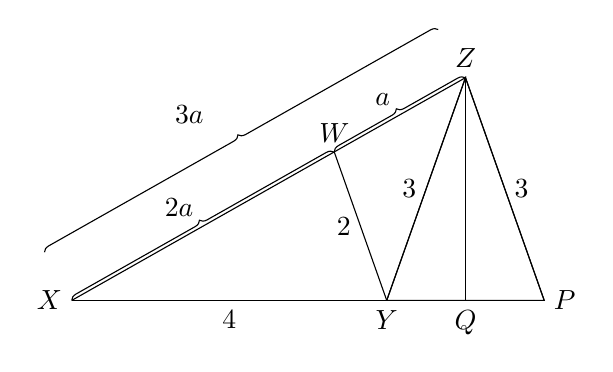
\begin{tikzpicture}[scale=1]
      \draw (0,0) -- (4,0) node [midway,below] {$4$};
      \draw (4,0) -- (5,2.82842712) node [midway,left] {$3$} -- (0,0);
      \draw (4,0) -- (3.33333333,1.88561808) node [midway, left] {$2$};
      \draw (3.33333333,1.88561808) node [above] {$W$};
      \draw (0,0) node [left] {$X$};
      \draw (4,0) node [below] {$Y$};
      \draw (5,2.82842712) node [above] {$Z$};
      \draw [decoration={brace,raise=0.0cm},decorate] (3.33333333,1.88561808)--(5,2.82842712) node [midway,above left] {$a$};
      \draw [decoration={brace,raise=0.0cm},decorate] (0,0)--(3.33333333,1.88561808) node [midway,above left] {$2a$};
      \draw [decoration={brace,raise=20pt},decorate] (0,0)--(5,2.82842712) node [midway,above left=20pt] {$3a$};

      \draw (6,0) node [right] {$P$};
      \draw (4,0)--(6,0)--(5,2.82842712)--cycle;
      \draw (5,2.82842712)--(6,0) node [midway,right] {$3$};

      \draw (5,0) node [below] {$Q$};
      \draw (5,2.82842712)--(5,0);
      \coordinate (Z) at (5,2.82842712);
      \coordinate (Q) at (5,0);
      \coordinate (Y) at (4,0);
      \tkzMarkRightAngle(Z,Q,Y)
    \end{tikzpicture}
  \end{center}
\end{frame}

\begin{frame}
  \begin{center}
    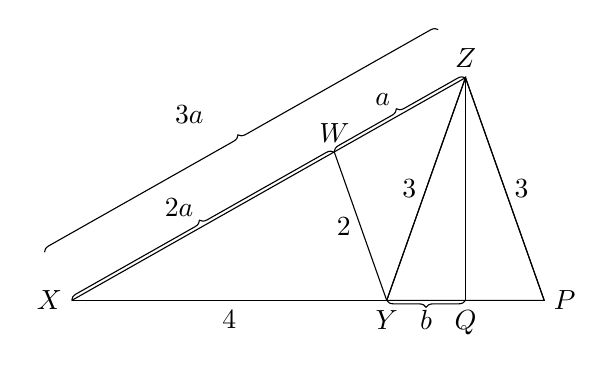
\begin{tikzpicture}[scale=1]
      \draw (0,0) -- (4,0) node [midway,below] {$4$};
      \draw (4,0) -- (5,2.82842712) node [midway,left] {$3$} -- (0,0);
      \draw (4,0) -- (3.33333333,1.88561808) node [midway, left] {$2$};
      \draw (3.33333333,1.88561808) node [above] {$W$};
      \draw (0,0) node [left] {$X$};
      \draw (4,0) node [below] {$Y$};
      \draw (5,2.82842712) node [above] {$Z$};
      \draw [decoration={brace,raise=0.0cm},decorate] (3.33333333,1.88561808)--(5,2.82842712) node [midway,above left] {$a$};
      \draw [decoration={brace,raise=0.0cm},decorate] (0,0)--(3.33333333,1.88561808) node [midway,above left] {$2a$};
      \draw [decoration={brace,raise=20pt},decorate] (0,0)--(5,2.82842712) node [midway,above left=20pt] {$3a$};

      \draw (6,0) node [right] {$P$};
      \draw (4,0)--(6,0)--(5,2.82842712)--cycle;
      \draw (5,2.82842712)--(6,0) node [midway,right] {$3$};

      \draw (5,0) node [below] {$Q$};
      \draw (5,2.82842712)--(5,0);
      \coordinate (Z) at (5,2.82842712);
      \coordinate (Q) at (5,0);
      \coordinate (Y) at (4,0);
      \tkzMarkRightAngle(Z,Q,Y)

      \draw [decoration={brace,mirror,raise=0cm},decorate] (4,0) -- (5,0) node [midway,below=0.0cm] {$b$};
    \end{tikzpicture}
  \end{center}
\end{frame}

\begin{frame}
  \begin{center}
    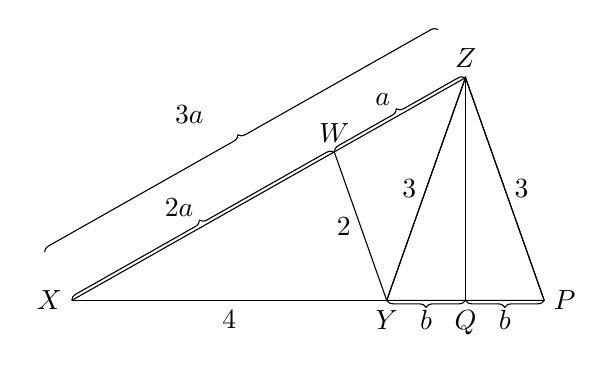
\begin{tikzpicture}[scale=1]
      \draw (0,0) node [left] {$X$};
      \draw (4,0) node [below] {$Y$};
      \draw (5,2.82842712) node [above] {$Z$};
      \draw (0,0) -- (4,0) node [midway,below] {$4$};
      \draw (4,0) -- (5,2.82842712) node [midway,left] {$3$} -- (0,0);

      \draw (3.33333333,1.88561808) node [above] {$W$};
      \draw (4,0) -- (3.33333333,1.88561808) node [midway, left] {$2$};

      \draw [decoration={brace,raise=0.0cm},decorate] (3.33333333,1.88561808)--(5,2.82842712) node [midway,above left] {$a$};
      \draw [decoration={brace,raise=0.0cm},decorate] (0,0)--(3.33333333,1.88561808) node [midway,above left] {$2a$};
      \draw [decoration={brace,raise=20pt},decorate] (0,0)--(5,2.82842712) node [midway,above left=20pt] {$3a$};

      \draw (6,0) node [right] {$P$};
      \draw (4,0)--(6,0)--(5,2.82842712)--cycle;
      \draw (5,2.82842712)--(6,0) node [midway,right] {$3$};

      \draw (5,0) node [below] {$Q$};
      \draw (5,2.82842712)--(5,0);
      \coordinate (Z) at (5,2.82842712);
      \coordinate (Q) at (5,0);
      \coordinate (Y) at (4,0);
      \tkzMarkRightAngle(Z,Q,Y)

      \draw [decoration={brace,mirror,raise=0cm},decorate] (4,0) -- (5,0) node [midway,below=0.0cm] {$b$};
      \draw [decoration={brace,mirror,raise=0cm},decorate] (5,0) -- (6,0) node [midway,below=0.0cm] {$b$};
    \end{tikzpicture}
  \end{center}
\end{frame}

\begin{frame}
  \begin{center}
    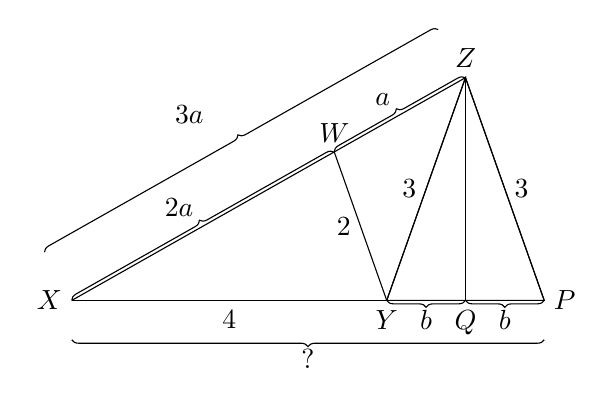
\begin{tikzpicture}[scale=1]
      \draw (0,0) node [left] {$X$};
      \draw (4,0) node [below] {$Y$};
      \draw (5,2.82842712) node [above] {$Z$};
      \draw (0,0) -- (4,0) node [midway,below] {$4$};
      \draw (4,0) -- (5,2.82842712) node [midway,left] {$3$} -- (0,0);

      \draw (3.33333333,1.88561808) node [above] {$W$};
      \draw (4,0) -- (3.33333333,1.88561808) node [midway, left] {$2$};

      \draw [decoration={brace,raise=0.0cm},decorate] (3.33333333,1.88561808)--(5,2.82842712) node [midway,above left] {$a$};
      \draw [decoration={brace,raise=0.0cm},decorate] (0,0)--(3.33333333,1.88561808) node [midway,above left] {$2a$};
      \draw [decoration={brace,raise=20pt},decorate] (0,0)--(5,2.82842712) node [midway,above left=20pt] {$3a$};

      \draw (6,0) node [right] {$P$};
      \draw (4,0)--(6,0)--(5,2.82842712)--cycle;
      \draw (5,2.82842712)--(6,0) node [midway,right] {$3$};

      \draw (5,0) node [below] {$Q$};
      \draw (5,2.82842712)--(5,0);
      \coordinate (Z) at (5,2.82842712);
      \coordinate (Q) at (5,0);
      \coordinate (Y) at (4,0);
      \tkzMarkRightAngle(Z,Q,Y)

      \draw [decoration={brace,mirror,raise=0cm},decorate] (4,0) -- (5,0) node [midway,below=0.0cm] {$b$};
      \draw [decoration={brace,mirror,raise=0cm},decorate] (5,0) -- (6,0) node [midway,below=0.0cm] {$b$};
      \draw [decoration={brace,mirror,raise=0.5cm},decorate] (0,0) -- (6,0) node [midway,below=0.5cm] {$?$};
    \end{tikzpicture}
  \end{center}
\end{frame}

\begin{frame}
  \begin{center}
    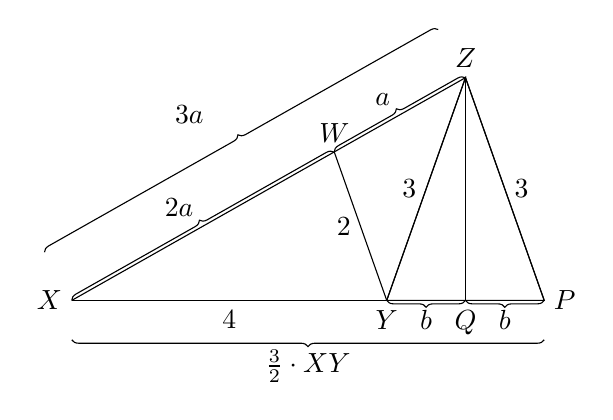
\begin{tikzpicture}[scale=1]
      \draw (0,0) node [left] {$X$};
      \draw (4,0) node [below] {$Y$};
      \draw (5,2.82842712) node [above] {$Z$};
      \draw (0,0) -- (4,0) node [midway,below] {$4$};
      \draw (4,0) -- (5,2.82842712) node [midway,left] {$3$} -- (0,0);

      \draw (3.33333333,1.88561808) node [above] {$W$};
      \draw (4,0) -- (3.33333333,1.88561808) node [midway, left] {$2$};

      \draw [decoration={brace,raise=0.0cm},decorate] (3.33333333,1.88561808)--(5,2.82842712) node [midway,above left] {$a$};
      \draw [decoration={brace,raise=0.0cm},decorate] (0,0)--(3.33333333,1.88561808) node [midway,above left] {$2a$};
      \draw [decoration={brace,raise=20pt},decorate] (0,0)--(5,2.82842712) node [midway,above left=20pt] {$3a$};

      \draw (6,0) node [right] {$P$};
      \draw (4,0)--(6,0)--(5,2.82842712)--cycle;
      \draw (5,2.82842712)--(6,0) node [midway,right] {$3$};

      \draw (5,0) node [below] {$Q$};
      \draw (5,2.82842712)--(5,0);
      \coordinate (Z) at (5,2.82842712);
      \coordinate (Q) at (5,0);
      \coordinate (Y) at (4,0);
      \tkzMarkRightAngle(Z,Q,Y)

      \draw [decoration={brace,mirror,raise=0cm},decorate] (4,0) -- (5,0) node [midway,below=0.0cm] {$b$};
      \draw [decoration={brace,mirror,raise=0cm},decorate] (5,0) -- (6,0) node [midway,below=0.0cm] {$b$};
      \draw [decoration={brace,mirror,raise=0.5cm},decorate] (0,0) -- (6,0) node [midway,below=0.5cm] {$\frac{3}{2}\cdot XY$};
    \end{tikzpicture}
  \end{center}
\end{frame}

\begin{frame}
  \begin{center}
    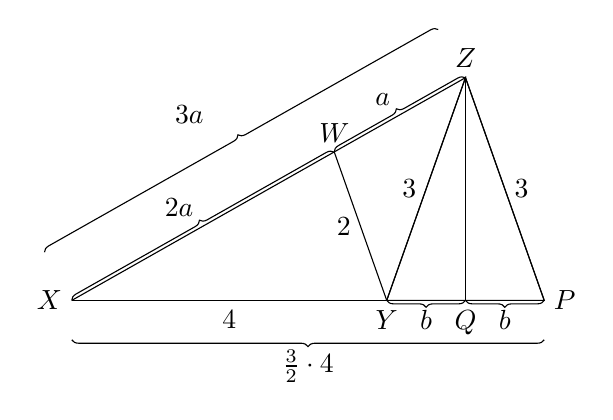
\begin{tikzpicture}[scale=1]
      \draw (0,0) node [left] {$X$};
      \draw (4,0) node [below] {$Y$};
      \draw (5,2.82842712) node [above] {$Z$};
      \draw (0,0) -- (4,0) node [midway,below] {$4$};
      \draw (4,0) -- (5,2.82842712) node [midway,left] {$3$} -- (0,0);

      \draw (3.33333333,1.88561808) node [above] {$W$};
      \draw (4,0) -- (3.33333333,1.88561808) node [midway, left] {$2$};

      \draw [decoration={brace,raise=0.0cm},decorate] (3.33333333,1.88561808)--(5,2.82842712) node [midway,above left] {$a$};
      \draw [decoration={brace,raise=0.0cm},decorate] (0,0)--(3.33333333,1.88561808) node [midway,above left] {$2a$};
      \draw [decoration={brace,raise=20pt},decorate] (0,0)--(5,2.82842712) node [midway,above left=20pt] {$3a$};

      \draw (6,0) node [right] {$P$};
      \draw (4,0)--(6,0)--(5,2.82842712)--cycle;
      \draw (5,2.82842712)--(6,0) node [midway,right] {$3$};

      \draw (5,0) node [below] {$Q$};
      \draw (5,2.82842712)--(5,0);
      \coordinate (Z) at (5,2.82842712);
      \coordinate (Q) at (5,0);
      \coordinate (Y) at (4,0);
      \tkzMarkRightAngle(Z,Q,Y)

      \draw [decoration={brace,mirror,raise=0cm},decorate] (4,0) -- (5,0) node [midway,below=0.0cm] {$b$};
      \draw [decoration={brace,mirror,raise=0cm},decorate] (5,0) -- (6,0) node [midway,below=0.0cm] {$b$};
      \draw [decoration={brace,mirror,raise=0.5cm},decorate] (0,0) -- (6,0) node [midway,below=0.5cm] {$\frac{3}{2}\cdot 4$};
    \end{tikzpicture}
  \end{center}
\end{frame}

\begin{frame}
  \begin{center}
    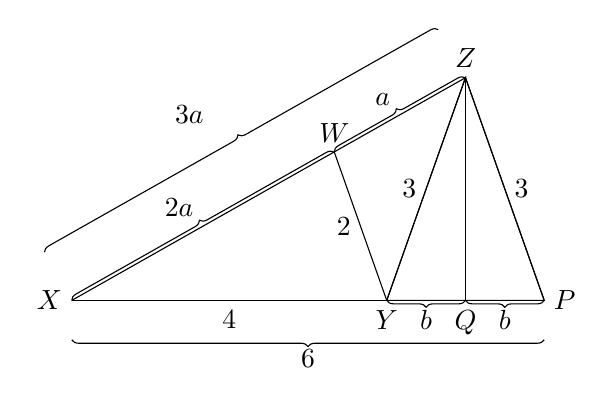
\begin{tikzpicture}[scale=1]
      \draw (0,0) node [left] {$X$};
      \draw (4,0) node [below] {$Y$};
      \draw (5,2.82842712) node [above] {$Z$};
      \draw (0,0) -- (4,0) node [midway,below] {$4$};
      \draw (4,0) -- (5,2.82842712) node [midway,left] {$3$} -- (0,0);

      \draw (3.33333333,1.88561808) node [above] {$W$};
      \draw (4,0) -- (3.33333333,1.88561808) node [midway, left] {$2$};

      \draw [decoration={brace,raise=0.0cm},decorate] (3.33333333,1.88561808)--(5,2.82842712) node [midway,above left] {$a$};
      \draw [decoration={brace,raise=0.0cm},decorate] (0,0)--(3.33333333,1.88561808) node [midway,above left] {$2a$};
      \draw [decoration={brace,raise=20pt},decorate] (0,0)--(5,2.82842712) node [midway,above left=20pt] {$3a$};

      \draw (6,0) node [right] {$P$};
      \draw (4,0)--(6,0)--(5,2.82842712)--cycle;
      \draw (5,2.82842712)--(6,0) node [midway,right] {$3$};

      \draw (5,0) node [below] {$Q$};
      \draw (5,2.82842712)--(5,0);
      \coordinate (Z) at (5,2.82842712);
      \coordinate (Q) at (5,0);
      \coordinate (Y) at (4,0);
      \tkzMarkRightAngle(Z,Q,Y)

      \draw [decoration={brace,mirror,raise=0cm},decorate] (4,0) -- (5,0) node [midway,below=0.0cm] {$b$};
      \draw [decoration={brace,mirror,raise=0cm},decorate] (5,0) -- (6,0) node [midway,below=0.0cm] {$b$};
      \draw [decoration={brace,mirror,raise=0.5cm},decorate] (0,0) -- (6,0) node [midway,below=0.5cm] {$6$};
    \end{tikzpicture}
  \end{center}
\end{frame}

\begin{frame}
  \begin{center}
    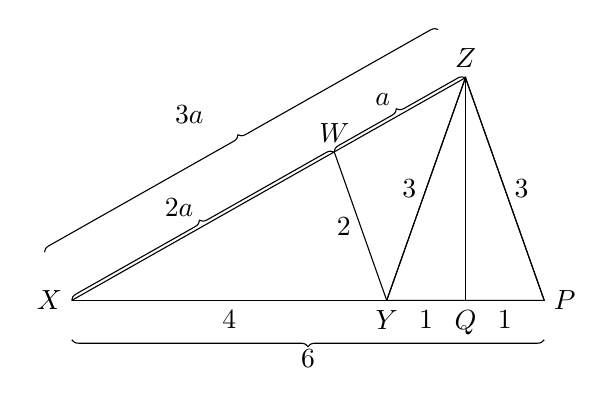
\begin{tikzpicture}[scale=1]
      \draw (0,0) node [left] {$X$};
      \draw (4,0) node [below] {$Y$};
      \draw (5,2.82842712) node [above] {$Z$};
      \draw (0,0) -- (4,0) node [midway,below] {$4$};
      \draw (4,0) -- (5,2.82842712) node [midway,left] {$3$} -- (0,0);

      \draw (3.33333333,1.88561808) node [above] {$W$};
      \draw (4,0) -- (3.33333333,1.88561808) node [midway, left] {$2$};

      \draw [decoration={brace,raise=0.0cm},decorate] (3.33333333,1.88561808)--(5,2.82842712) node [midway,above left] {$a$};
      \draw [decoration={brace,raise=0.0cm},decorate] (0,0)--(3.33333333,1.88561808) node [midway,above left] {$2a$};
      \draw [decoration={brace,raise=20pt},decorate] (0,0)--(5,2.82842712) node [midway,above left=20pt] {$3a$};

      \draw (6,0) node [right] {$P$};
      \draw (4,0)--(6,0)--(5,2.82842712)--cycle;
      \draw (5,2.82842712)--(6,0) node [midway,right] {$3$};

      \draw (5,0) node [below] {$Q$};
      \draw (5,2.82842712)--(5,0);
      \coordinate (Z) at (5,2.82842712);
      \coordinate (Q) at (5,0);
      \coordinate (Y) at (4,0);
      \tkzMarkRightAngle(Z,Q,Y)

      \draw (4,0) -- (5,0) node [midway,below=0.0cm] {$1$};
      \draw (5,0) -- (6,0) node [midway,below=0.0cm] {$1$};
      \draw [decoration={brace,mirror,raise=0.5cm},decorate] (0,0) -- (6,0) node [midway,below=0.5cm] {$6$};
    \end{tikzpicture}
  \end{center}
\end{frame}

\begin{frame}
  \begin{center}
    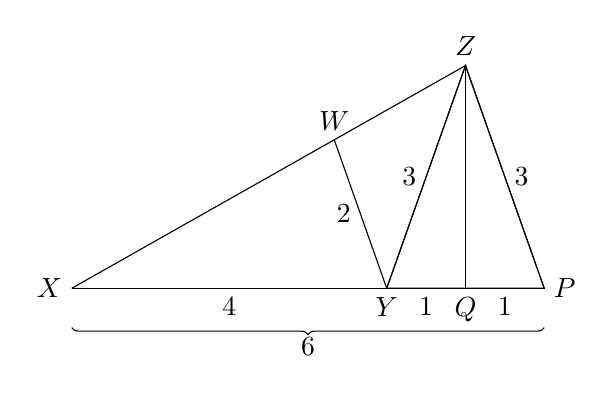
\begin{tikzpicture}[scale=1]
      \draw (0,0) node [left] {$X$};
      \draw (4,0) node [below] {$Y$};
      \draw (5,2.82842712) node [above] {$Z$};
      \draw (0,0) -- (4,0) node [midway,below] {$4$};
      \draw (4,0) -- (5,2.82842712) node [midway,left] {$3$} -- (0,0);

      \draw (3.33333333,1.88561808) node [above] {$W$};
      \draw (4,0) -- (3.33333333,1.88561808) node [midway, left] {$2$};

      \draw (6,0) node [right] {$P$};
      \draw (4,0)--(6,0)--(5,2.82842712)--cycle;
      \draw (5,2.82842712)--(6,0) node [midway,right] {$3$};

      \draw (5,0) node [below] {$Q$};
      \draw (5,2.82842712)--(5,0);
      \coordinate (Z) at (5,2.82842712);
      \coordinate (Q) at (5,0);
      \coordinate (Y) at (4,0);
      \tkzMarkRightAngle(Z,Q,Y)

      \draw (4,0) -- (5,0) node [midway,below=0.0cm] {$1$};
      \draw (5,0) -- (6,0) node [midway,below=0.0cm] {$1$};
      \draw [decoration={brace,mirror,raise=0.5cm},decorate] (0,0) -- (6,0) node [midway,below=0.5cm] {$6$};
    \end{tikzpicture}
  \end{center}
\end{frame}

\begin{frame}
  \begin{center}
    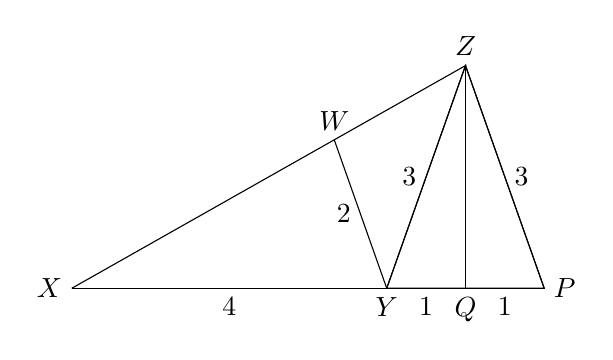
\begin{tikzpicture}[scale=1]
      \draw (0,0) node [left] {$X$};
      \draw (4,0) node [below] {$Y$};
      \draw (5,2.82842712) node [above] {$Z$};
      \draw (0,0) -- (4,0) node [midway,below] {$4$};
      \draw (4,0) -- (5,2.82842712) node [midway,left] {$3$} -- (0,0);

      \draw (3.33333333,1.88561808) node [above] {$W$};
      \draw (4,0) -- (3.33333333,1.88561808) node [midway, left] {$2$};

      \draw (6,0) node [right] {$P$};
      \draw (4,0)--(6,0)--(5,2.82842712)--cycle;
      \draw (5,2.82842712)--(6,0) node [midway,right] {$3$};

      \draw (5,0) node [below] {$Q$};
      \draw (5,2.82842712)--(5,0);
      \coordinate (Z) at (5,2.82842712);
      \coordinate (Q) at (5,0);
      \coordinate (Y) at (4,0);
      \tkzMarkRightAngle(Z,Q,Y)

      \draw (4,0) -- (5,0) node [midway,below=0.0cm] {$1$};
      \draw (5,0) -- (6,0) node [midway,below=0.0cm] {$1$};
    \end{tikzpicture}
  \end{center}
\end{frame}

\begin{frame}
  \begin{center}
    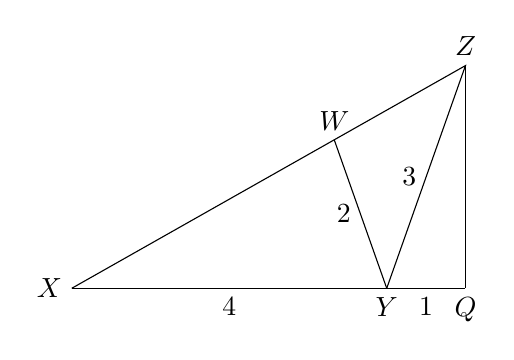
\begin{tikzpicture}[scale=1]
      \draw (0,0) node [left] {$X$};
      \draw (4,0) node [below] {$Y$};
      \draw (5,2.82842712) node [above] {$Z$};
      \draw (0,0) -- (4,0) node [midway,below] {$4$};
      \draw (4,0) -- (5,2.82842712) node [midway,left] {$3$} -- (0,0);

      \draw (3.33333333,1.88561808) node [above] {$W$};
      \draw (4,0) -- (3.33333333,1.88561808) node [midway, left] {$2$};

      \draw (5,0) node [below] {$Q$};
      \draw (5,2.82842712)--(5,0);
      \coordinate (Z) at (5,2.82842712);
      \coordinate (Q) at (5,0);
      \coordinate (Y) at (4,0);
      \tkzMarkRightAngle(Z,Q,Y)
      \draw (4,0) -- (5,0) node [midway,below=0.0cm] {$1$};
    \end{tikzpicture}
  \end{center}
\end{frame}

\begin{frame}
  \begin{center}
    \begin{tikzpicture}[scale=1]
      \draw (0,0) node [left] {$X$};
      \draw (4,0) node [below] {$Y$};
      \draw (5,2.82842712) node [above] {$Z$};
      \draw (0,0) -- (4,0) node [midway,below] {$4$};
      \draw (4,0) -- (5,2.82842712) node [midway,left] {$3$} -- (0,0);

      \draw (5,0) node [below] {$Q$};
      \draw (5,2.82842712)--(5,0);
      \coordinate (Z) at (5,2.82842712);
      \coordinate (Q) at (5,0);
      \coordinate (Y) at (4,0);
      \tkzMarkRightAngle(Z,Q,Y)
      \draw (4,0) -- (5,0) node [midway,below=0.0cm] {$1$};
    \end{tikzpicture}
  \end{center}
\end{frame}

\begin{frame}
  \begin{center}
    \begin{tikzpicture}[scale=1]
      \draw (0,0) node [left] {$X$};
      \draw (4,0) node [below] {$Y$};
      \draw (5,2.82842712) node [above] {$Z$};
      \draw (0,0) -- (4,0) node [midway,below] {$4$};
      \draw (4,0) -- (5,2.82842712) node [midway,left] {$3$} -- (0,0);

      \draw (5,0) node [below] {$Q$};
      \draw (5,2.82842712)--(5,0);
      \coordinate (Z) at (5,2.82842712);
      \coordinate (Q) at (5,0);
      \coordinate (Y) at (4,0);
      \tkzMarkRightAngle(Z,Q,Y)
      \draw (4,0) -- (5,0) node [midway,below=0.0cm] {$1$};
    \end{tikzpicture}
  \end{center}
  By Pythagorean theorem,
  \[
    XZ^2 = XQ^2 + QZ^2
  \]
\end{frame}

\begin{frame}
  \begin{center}
    \begin{tikzpicture}[scale=1]
      \draw (0,0) node [left] {$X$};
      \draw (4,0) node [below] {$Y$};
      \draw (5,2.82842712) node [above] {$Z$};
      \draw (0,0) -- (4,0) node [midway,below] {$4$};
      \draw (4,0) -- (5,2.82842712) node [midway,left] {$3$} -- (0,0);

      \draw (5,0) node [below] {$Q$};
      \draw (5,2.82842712)--(5,0);
      \coordinate (Z) at (5,2.82842712);
      \coordinate (Q) at (5,0);
      \coordinate (Y) at (4,0);
      \tkzMarkRightAngle(Z,Q,Y)
      \draw (4,0) -- (5,0) node [midway,below=0.0cm] {$1$};
    \end{tikzpicture}
  \end{center}
  By Pythagorean theorem,
  \[
    XZ^2 = XQ^2 + (YZ^2 - YQ^2)
  \]
\end{frame}

\begin{frame}
  \begin{center}
    \begin{tikzpicture}[scale=1]
      \draw (0,0) node [left] {$X$};
      \draw (4,0) node [below] {$Y$};
      \draw (5,2.82842712) node [above] {$Z$};
      \draw (0,0) -- (4,0) node [midway,below] {$4$};
      \draw (4,0) -- (5,2.82842712) node [midway,left] {$3$} -- (0,0);

      \draw (5,0) node [below] {$Q$};
      \draw (5,2.82842712)--(5,0);
      \coordinate (Z) at (5,2.82842712);
      \coordinate (Q) at (5,0);
      \coordinate (Y) at (4,0);
      \tkzMarkRightAngle(Z,Q,Y)
      \draw (4,0) -- (5,0) node [midway,below=0.0cm] {$1$};
    \end{tikzpicture}
  \end{center}
  \[
    XZ^2 = XQ^2 + (YZ^2 - YQ^2)
  \]
\end{frame}

\begin{frame}
  \begin{center}
    \begin{tikzpicture}[scale=1]
      \draw (0,0) node [left] {$X$};
      \draw (4,0) node [below] {$Y$};
      \draw (5,2.82842712) node [above] {$Z$};
      \draw (0,0) -- (4,0) node [midway,below] {$4$};
      \draw (4,0) -- (5,2.82842712) node [midway,left] {$3$} -- (0,0);

      \draw (5,0) node [below] {$Q$};
      \draw (5,2.82842712)--(5,0);
      \coordinate (Z) at (5,2.82842712);
      \coordinate (Q) at (5,0);
      \coordinate (Y) at (4,0);
      \tkzMarkRightAngle(Z,Q,Y)
      \draw (4,0) -- (5,0) node [midway,below=0.0cm] {$1$};
    \end{tikzpicture}
  \end{center}
  \[
    XZ^2 = (XY+YQ)^2 + (YZ^2 - YQ^2)
  \]
\end{frame}

\begin{frame}
  \begin{center}
    \begin{tikzpicture}[scale=1]
      \draw (0,0) node [left] {$X$};
      \draw (4,0) node [below] {$Y$};
      \draw (5,2.82842712) node [above] {$Z$};
      \draw (0,0) -- (4,0) node [midway,below] {$4$};
      \draw (4,0) -- (5,2.82842712) node [midway,left] {$3$} -- (0,0);

      \draw (5,0) node [below] {$Q$};
      \draw (5,2.82842712)--(5,0);
      \coordinate (Z) at (5,2.82842712);
      \coordinate (Q) at (5,0);
      \coordinate (Y) at (4,0);
      \tkzMarkRightAngle(Z,Q,Y)
      \draw (4,0) -- (5,0) node [midway,below=0.0cm] {$1$};
    \end{tikzpicture}
  \end{center}
  \[
    XZ^2 = (4+YQ)^2 + (YZ^2 - YQ^2)
  \]
\end{frame}

\begin{frame}
  \begin{center}
    \begin{tikzpicture}[scale=1]
      \draw (0,0) node [left] {$X$};
      \draw (4,0) node [below] {$Y$};
      \draw (5,2.82842712) node [above] {$Z$};
      \draw (0,0) -- (4,0) node [midway,below] {$4$};
      \draw (4,0) -- (5,2.82842712) node [midway,left] {$3$} -- (0,0);

      \draw (5,0) node [below] {$Q$};
      \draw (5,2.82842712)--(5,0);
      \coordinate (Z) at (5,2.82842712);
      \coordinate (Q) at (5,0);
      \coordinate (Y) at (4,0);
      \tkzMarkRightAngle(Z,Q,Y)
      \draw (4,0) -- (5,0) node [midway,below=0.0cm] {$1$};
    \end{tikzpicture}
  \end{center}
  \[
    XZ^2 = (4+1)^2 + (YZ^2 - 1^2)
  \]
\end{frame}

\begin{frame}
  \begin{center}
    \begin{tikzpicture}[scale=1]
      \draw (0,0) node [left] {$X$};
      \draw (4,0) node [below] {$Y$};
      \draw (5,2.82842712) node [above] {$Z$};
      \draw (0,0) -- (4,0) node [midway,below] {$4$};
      \draw (4,0) -- (5,2.82842712) node [midway,left] {$3$} -- (0,0);

      \draw (5,0) node [below] {$Q$};
      \draw (5,2.82842712)--(5,0);
      \coordinate (Z) at (5,2.82842712);
      \coordinate (Q) at (5,0);
      \coordinate (Y) at (4,0);
      \tkzMarkRightAngle(Z,Q,Y)
      \draw (4,0) -- (5,0) node [midway,below=0.0cm] {$1$};
    \end{tikzpicture}
  \end{center}
  \[
    XZ^2 = (4+1)^2 + (3^2 - 1^2)
  \]
\end{frame}

\begin{frame}
  \begin{center}
    \begin{tikzpicture}[scale=1]
      \draw (0,0) node [left] {$X$};
      \draw (4,0) node [below] {$Y$};
      \draw (5,2.82842712) node [above] {$Z$};
      \draw (0,0) -- (4,0) node [midway,below] {$4$};
      \draw (4,0) -- (5,2.82842712) node [midway,left] {$3$} -- (0,0);

      \draw (5,0) node [below] {$Q$};
      \draw (5,2.82842712)--(5,0);
      \coordinate (Z) at (5,2.82842712);
      \coordinate (Q) at (5,0);
      \coordinate (Y) at (4,0);
      \tkzMarkRightAngle(Z,Q,Y)
      \draw (4,0) -- (5,0) node [midway,below=0.0cm] {$1$};
    \end{tikzpicture}
  \end{center}
  \[
    XZ^2 = 5^2 + (3^2 - 1^2)
  \]
\end{frame}

\begin{frame}
  \begin{center}
    \begin{tikzpicture}[scale=1]
      \draw (0,0) node [left] {$X$};
      \draw (4,0) node [below] {$Y$};
      \draw (5,2.82842712) node [above] {$Z$};
      \draw (0,0) -- (4,0) node [midway,below] {$4$};
      \draw (4,0) -- (5,2.82842712) node [midway,left] {$3$} -- (0,0);

      \draw (5,0) node [below] {$Q$};
      \draw (5,2.82842712)--(5,0);
      \coordinate (Z) at (5,2.82842712);
      \coordinate (Q) at (5,0);
      \coordinate (Y) at (4,0);
      \tkzMarkRightAngle(Z,Q,Y)
      \draw (4,0) -- (5,0) node [midway,below=0.0cm] {$1$};
    \end{tikzpicture}
  \end{center}
  \[
    XZ^2 = 25 + (3^2 - 1^2)
  \]
\end{frame}

\begin{frame}
  \begin{center}
    \begin{tikzpicture}[scale=1]
      \draw (0,0) node [left] {$X$};
      \draw (4,0) node [below] {$Y$};
      \draw (5,2.82842712) node [above] {$Z$};
      \draw (0,0) -- (4,0) node [midway,below] {$4$};
      \draw (4,0) -- (5,2.82842712) node [midway,left] {$3$} -- (0,0);

      \draw (5,0) node [below] {$Q$};
      \draw (5,2.82842712)--(5,0);
      \coordinate (Z) at (5,2.82842712);
      \coordinate (Q) at (5,0);
      \coordinate (Y) at (4,0);
      \tkzMarkRightAngle(Z,Q,Y)
      \draw (4,0) -- (5,0) node [midway,below=0.0cm] {$1$};
    \end{tikzpicture}
  \end{center}
  \[
    XZ^2 = 25 + (9 - 1^2)
  \]
\end{frame}

\begin{frame}
  \begin{center}
    \begin{tikzpicture}[scale=1]
      \draw (0,0) node [left] {$X$};
      \draw (4,0) node [below] {$Y$};
      \draw (5,2.82842712) node [above] {$Z$};
      \draw (0,0) -- (4,0) node [midway,below] {$4$};
      \draw (4,0) -- (5,2.82842712) node [midway,left] {$3$} -- (0,0);

      \draw (5,0) node [below] {$Q$};
      \draw (5,2.82842712)--(5,0);
      \coordinate (Z) at (5,2.82842712);
      \coordinate (Q) at (5,0);
      \coordinate (Y) at (4,0);
      \tkzMarkRightAngle(Z,Q,Y)
      \draw (4,0) -- (5,0) node [midway,below=0.0cm] {$1$};
    \end{tikzpicture}
  \end{center}
  \[
    XZ^2 = 25 + (9 - 1)
  \]
\end{frame}

\begin{frame}
  \begin{center}
    \begin{tikzpicture}[scale=1]
      \draw (0,0) node [left] {$X$};
      \draw (4,0) node [below] {$Y$};
      \draw (5,2.82842712) node [above] {$Z$};
      \draw (0,0) -- (4,0) node [midway,below] {$4$};
      \draw (4,0) -- (5,2.82842712) node [midway,left] {$3$} -- (0,0);

      \draw (5,0) node [below] {$Q$};
      \draw (5,2.82842712)--(5,0);
      \coordinate (Z) at (5,2.82842712);
      \coordinate (Q) at (5,0);
      \coordinate (Y) at (4,0);
      \tkzMarkRightAngle(Z,Q,Y)
      \draw (4,0) -- (5,0) node [midway,below=0.0cm] {$1$};
    \end{tikzpicture}
  \end{center}
  \[
    XZ^2 = 25 + 8
  \]
\end{frame}

\begin{frame}
  \begin{center}
    \begin{tikzpicture}[scale=1]
      \draw (0,0) node [left] {$X$};
      \draw (4,0) node [below] {$Y$};
      \draw (5,2.82842712) node [above] {$Z$};
      \draw (0,0) -- (4,0) node [midway,below] {$4$};
      \draw (4,0) -- (5,2.82842712) node [midway,left] {$3$} -- (0,0);

      \draw (5,0) node [below] {$Q$};
      \draw (5,2.82842712)--(5,0);
      \coordinate (Z) at (5,2.82842712);
      \coordinate (Q) at (5,0);
      \coordinate (Y) at (4,0);
      \tkzMarkRightAngle(Z,Q,Y)
      \draw (4,0) -- (5,0) node [midway,below=0.0cm] {$1$};
    \end{tikzpicture}
  \end{center}
  \[
    XZ^2 = \boxed{33}
  \]
\end{frame}

%\draw [decoration={brace,raise=0cm},decorate] (5,2.82842712)--(5,0) node [midway,right] {$?$};

\section{Reflection}

\subsection*{Review the concepts.}

\begin{frame}
  \frametitle{Concepts}
  %\framesubtitle{What?}
  \pause
  \begin{itemize}
    \item similar triangles \pause
    \item properties of isosceles triangles \pause
    \item Pythagorean theorem
  \end{itemize}
\end{frame}

\begin{comment}
\subsection*{A message from Tim.}

\tcbset{colframe=ml3}

\begin{frame}
  %\frametitle{A message from Tim.}
  \begin{center}
    \begin{figure}
      \tcbox{\includegraphics[scale=0.20]{sanders.png}}
      ``Hi everybody, this is Tim.''
    \end{figure}
  \end{center}
\end{frame}
\end{comment}

\end{document}